\documentclass[11pt,a4paper]{report}
\usepackage[utf8]{inputenc}
\usepackage[french]{babel}
\usepackage[T1]{fontenc}
\usepackage{amsmath}
\usepackage{amsfonts}
\usepackage{amssymb}
\usepackage{listings}
\usepackage{caption}
\usepackage{alltt}
%\usepackage{picins}
\usepackage{color}
\usepackage[left=2cm,right=2cm,top=2cm,bottom=2cm]{geometry}
\usepackage{hyperref}
\usepackage{graphicx}
\author{Damien Hostettler, Simon Maurel, Qi Chen et Vicky Dincher}
\title{Rapport de projet Sémantique et Traduction des langages} 
\date{17 Juin 2016}

\renewcommand{\thesection}{\arabic{section}}
\setcounter{tocdepth}{3}
\begin{document}
\maketitle
\tableofcontents
\newpage
 
\section*{Introduction}

Le but de ce projet a été de réaliser un compilateur pour les langages $\mu C$ et $\mu C \#$. Ce compilateur doit vérifier les erreurs détectables lors de la compilation (erreurs de types, variable non définies ...) et doit générer la traduction du programme compilé en langage \textbf{TAM}.\\
La réalisation de ce compilateur passe passe par la gestion de la table des symboles, des erreurs de type, ainsi que la génération de code


\section{Construction de la table des symboles}

La table des symboles doit contenir toutes les informations sur ce qui est déclaré dans le programme (variables, types, fonction) sauf leur valeur en temps réel. \\
Une table des symboles est une liste d'élément de type \textsc{info} que l'on peut repérer par leur nom (nom de variable par exemple).

\subsection{Contenu et hiérarchie}

Nous avons donc modélisé notre table comme un $HashMap<String$,\textsc{infovar}$>$.
Ce sont les différents couples (Nom des variables (fonctions ...), informations liées).\\
On trouve ainsi plusieurs type d'informations (toutes héritées de la classe \textsc{info}): 
\begin{itemize}
\item Les \textsc{infovar} liées au variables. Elles contiennent simplement le type de la variable, et son emplacement dans la pile. 
\item Les \textsc{infotype} liées aux types créés avec $typedef$. Elles contiennent un type (celui créé). 
\item Les \textsc{infofonc}, liées aux fonctions. Elles contiennent le type de retour de la fonction, la liste des différentes possibilités de paramètres pouvant être utilisés avec cette fonction (surcharges), ainsi qu'une TDS fille de la TDS courante, contenant les informations sur les variables (ou types) locales à la fonction. 
\end{itemize}



On crée donc une TDS fille à chaque nouvelle fonction, mais également lorsque l'on rentre dans un nouveau bloc. On obtient ainsi la hiérarchie suivante: \\\\

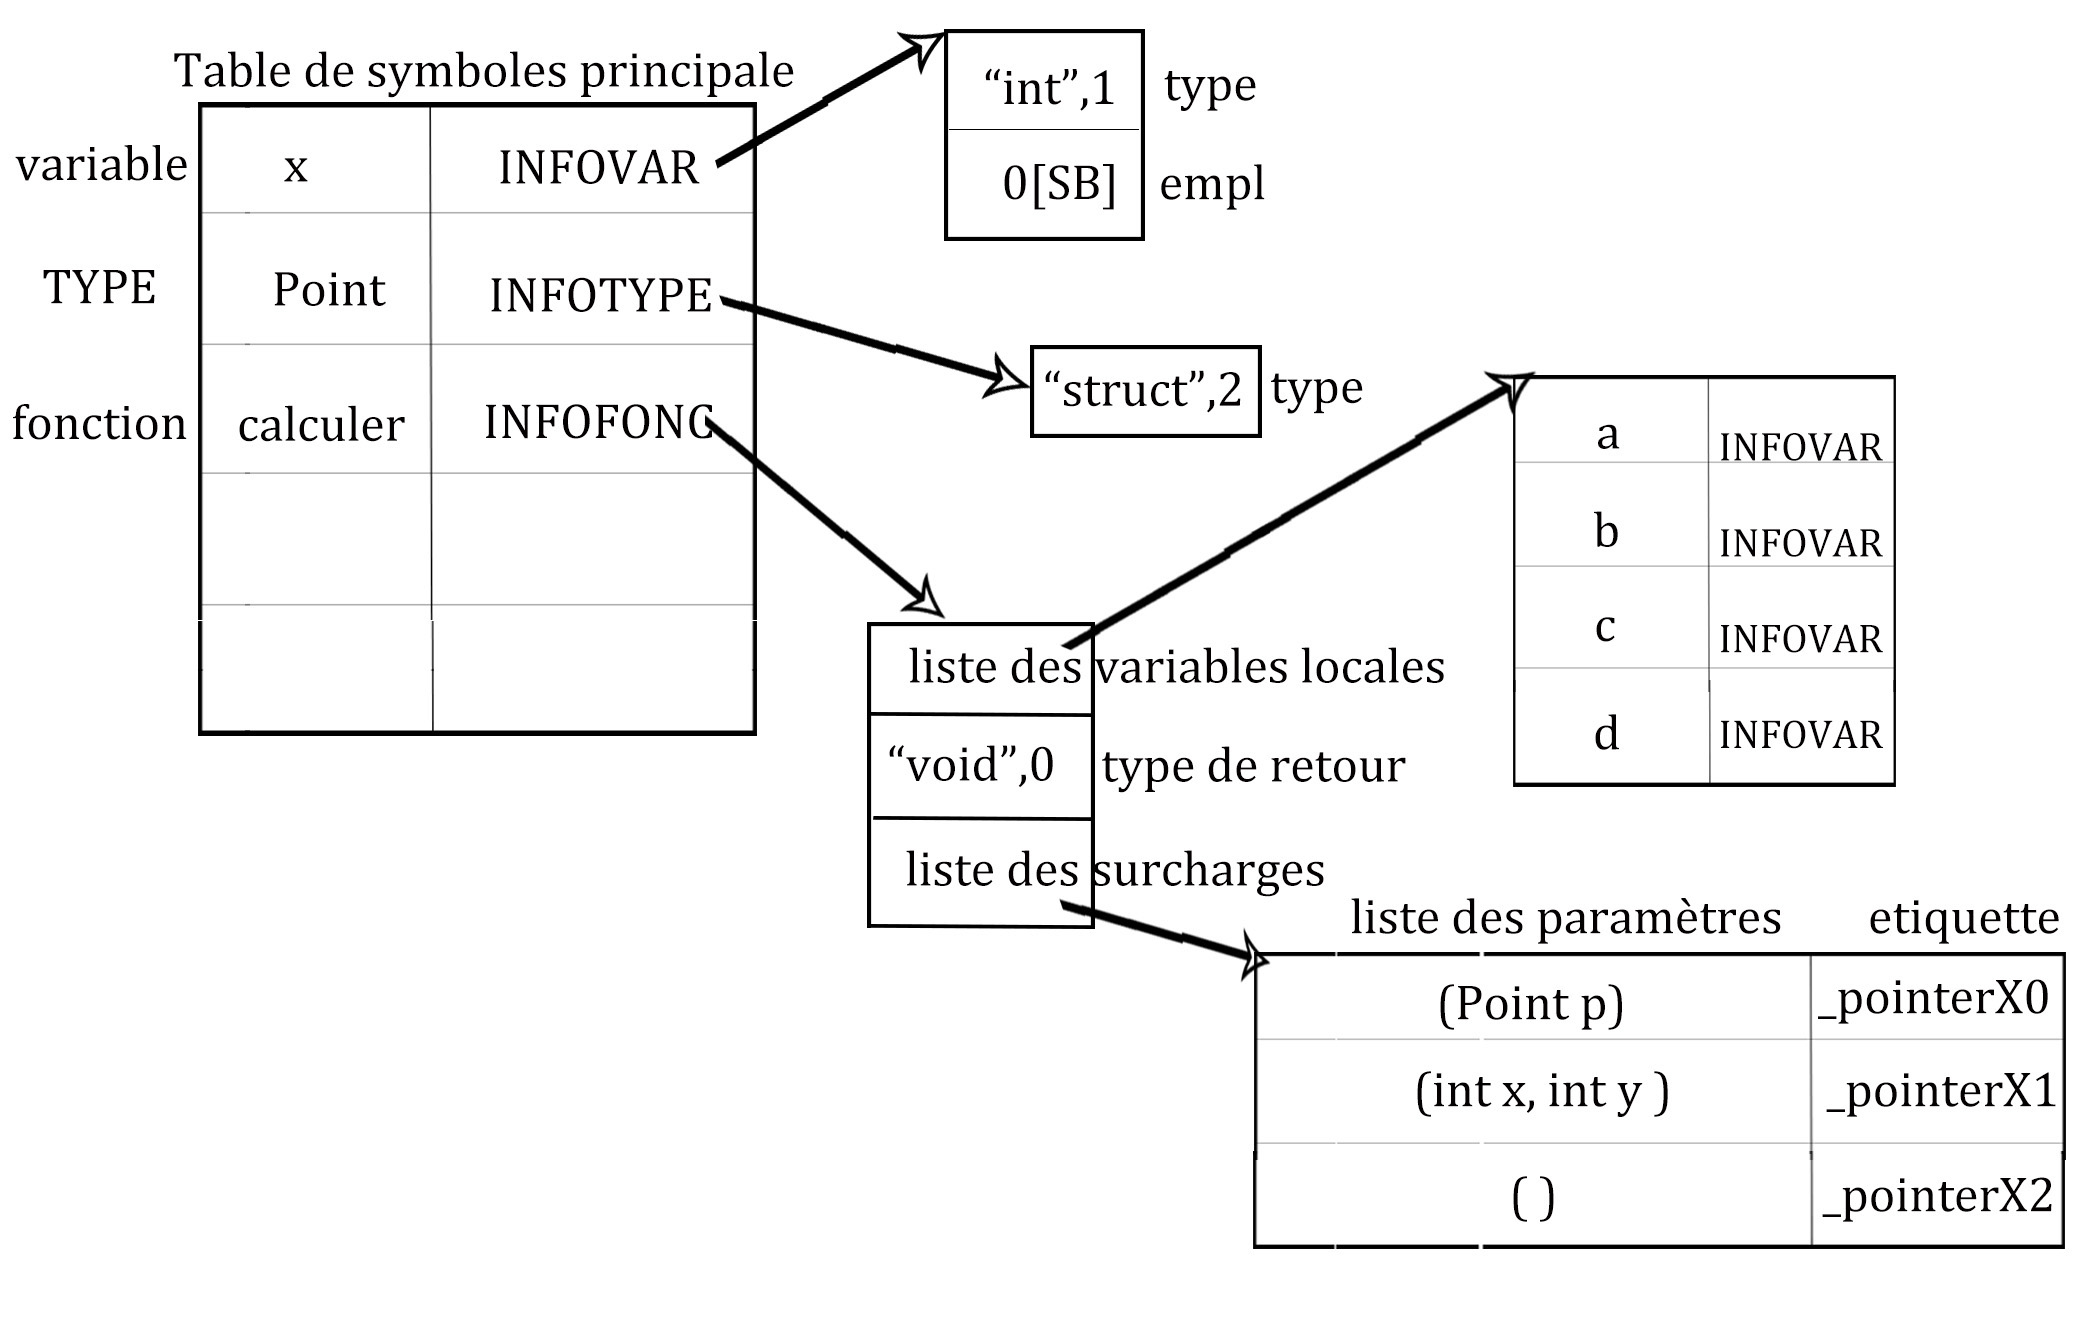
\includegraphics[scale=0.2]{structureMicroC.jpg}

\subsection{Gestion des variables globales}

Le compilateur implémenté permet l'utilisation de variables globales (déclarées tout au début du programme). Pour ce faire, l'emplacement des variables globales au programme (qui ne sont pas déclarées à l'intérieur d'un bloc) se situera dans le registre {\bf SB}, et les variables locales seront déclarées dans le registre {\bf LB}.

\subsection{Ajouts pour le $\mu C \#$}

Les notions de  $namespace$ et de $classe$ ont été ajoutées dans le langage $\mu C \#$. On aura ainsi des \textsc{infonamespace} qui peuvent être présents dans la TDS. Les namespaces ne sont pas gérés dans notre programme.\\

Afin de représenter une classe, nous avons créé le type \textsc{object} qui hérite de \textsc{dtype}. 
Ainsi, un \textsc{object} contient une \textsc{tds}, qui est initialisée par: 
\begin{itemize}
\item Une \textsc{tds} vide si la classe déclarée est la classe mère (classe objet). 
\item Une \textsc{tds} fille de la \textsc{tds} de la classe mère, si la classe considérée est héritée.
\end{itemize}

La taille de notre classe est définie par la taille de tous ses attributs (comme dans le cas d'un \textsc{struct}). Ainsi, on définit la taille à la fin de la définition d'une classe, avec une recherche de chaque attribut dans la \textsc{tds} de la classe. \\\\
Un \textsc{object} possède également son héritage (de type \textsc{object}) qui sera null si une classe ne possède pas d'héritage.


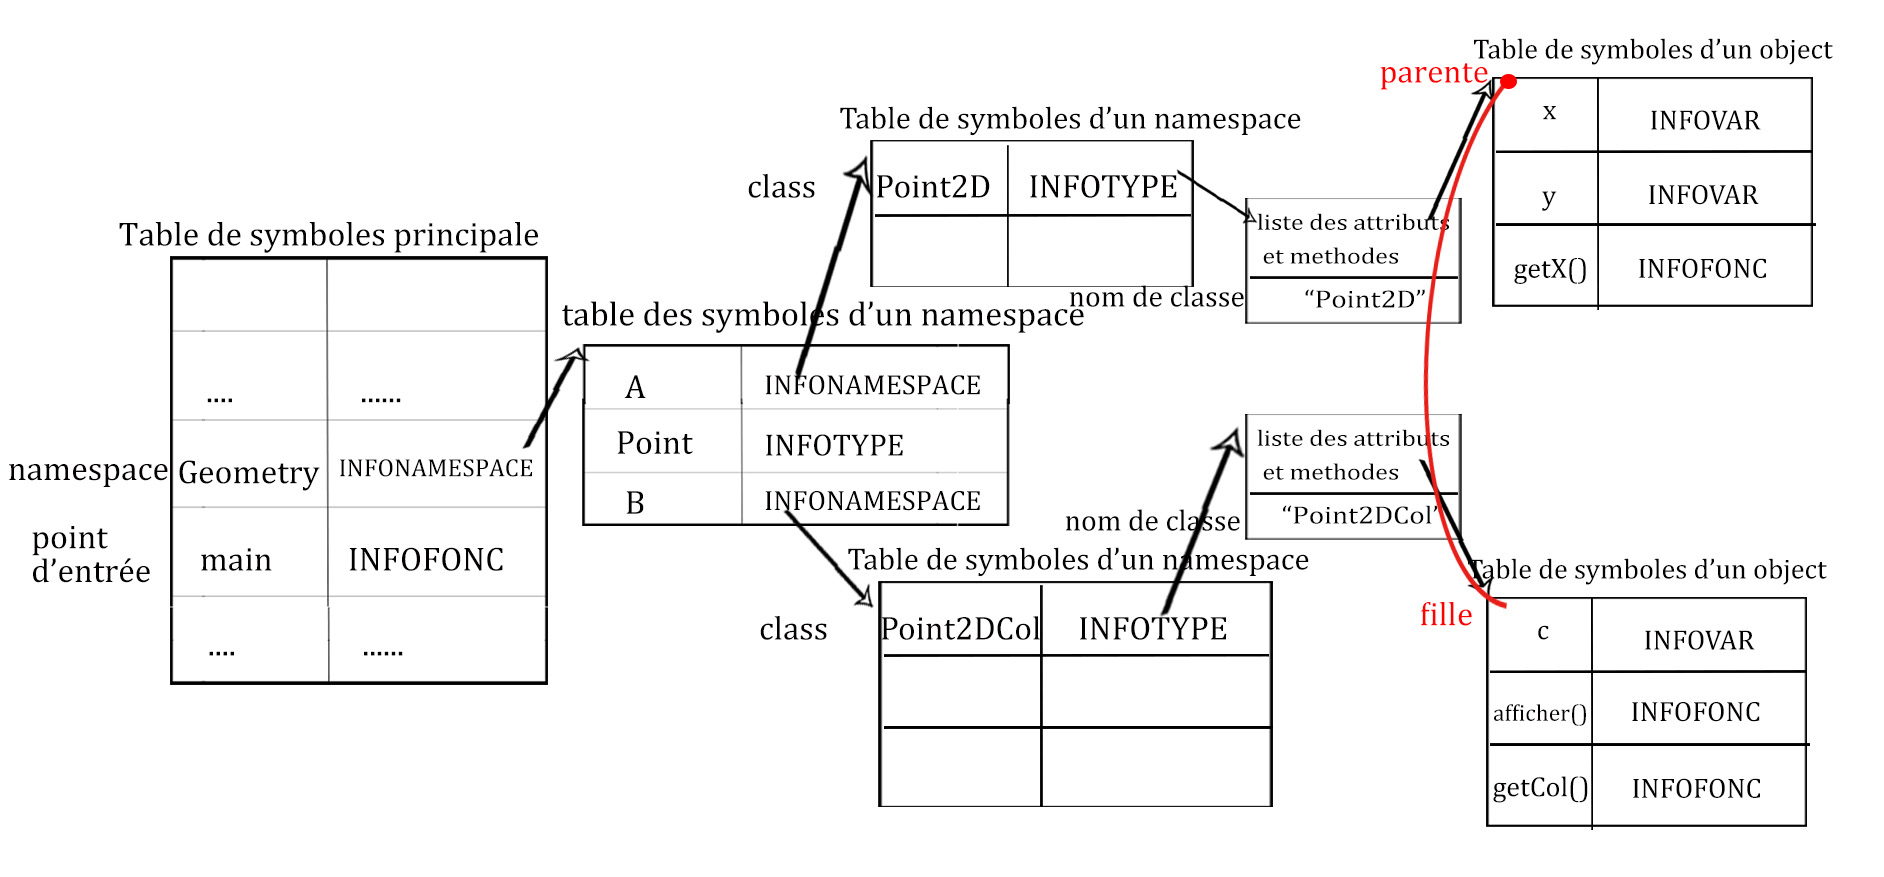
\includegraphics[scale=0.25]{microCsharp.jpg}



\section{Préconditions et gestions des erreurs de type}

Pour la gestion des types et des erreurs de types, nous avons imposé certaines conditions, notamment pour la compatibilité des opérateurs. Dans la gestion des opérateurs, on prend en compte le type {\bf bool}, pris en compte dans le langage $\mu C \#$.


\subsection{Opérateurs et compatibilité de types}

\begin{itemize}
\item Les opérateurs de comparaison $\leq$, $\geq$ ,$<$,$>$,$+$ (unaire), $-$ (unaire), $-$ (binaire), $*$, $/$, $\%$ ne sont compatible qu'avec les types \textbf{ int}.
\item Les opérateurs $=$ et $\neq$  sont compatible avec les types {\bf int} et {\bf char}.
\item L'opérateur $+$ est compatible avec les types {\bf int}, {\bf string } et {\bf char }.
\item Les opérateurs $\vee,\wedge,$ $not$ sont compatibles avec les opérateurs {\bf int } et {\bf bool }.
\end{itemize}

Ainsi, afin de pouvoir gérer les types lors des opérations sur des variables, nous avons créé le type Opérateur, qui affecte à chaque numéro d'opérateurs (numérotés de 1 à 15) une liste des noms des types admis.\\
 On peut ainsi tester la compatibilité d'un type pour un opérateur dans la classe DTYPE. On peut donc effectuer une opération à condition que les deux opérandes aient le même type, et que ce type soit compatible avec celui de l'opérateur. Sinon, on renvoie une erreur.



\subsection{Types particuliers}

 Les types particuliers comme les \textsc{pointeurs} et les \textsc{structs} ont été géré de la même manière qu'en TP.

\section{Fonctions et leurs surcharges}

Les fonctions ont été implémentées de manière à pouvoir les surcharger $i.e$: on peut appeler une fonction avec plusieurs listes de paramètres différentes, mais {\bf le type de retour doit toujours rester le même}. Pour ce faire, nous avons implémenté les fonctions de la manière suivante: \\
Une \textsc{infofonc} contient une liste de \textsc{surcharges}. \\
Une \textsc{surcharge} est une liste d'\textsc{infovar} ainsi que l'étiquette associée à la surcharge (ce sera dans notre cas \textsl{nom$\_$fonctionXnum$\_$surcharge}  \\\\
Ainsi, lors de la déclaration d'une fonction, on réalise les actions suivantes: 
\begin{alltt}
INFO i = TDS.RechercherGlobalement(nom_fonction)
  {\bf Si} i = null {\bf alors}
      Créer une nouvelle INFOFONC, avec la surcharge correspondante aux 
      paramètres déclarés associée au numéro X0
  {\bf Sinon}
      Vérifier que i est bien une INFOFONC
      Ajouter la surcharge des paramètres déclarés aux autres surcharges,
      associée à un nouveau numéro
  {\bf Fin si} 
\end{alltt}

Ainsi, lors de l'appel, on génère une liste ordonnée de types (correspondante aux paramètres avec lesquels la fonction est appelée), et on la compare avec chacune des surcharges de la fonction (dont l'info est obtenue grâce au nom). \\ 
Si l'une des surcharges correspond, on appelle la fonction avec cette surcharge.

\section{Génération de code}

La génération de code a été gérée de la même façon qu'en TP, mais quelques ajouts ont été faits.

\subsection{Opérateurs}

Afin de réaliser les différentes opérations, nous avons créé la fonction 
$GenSubr$ dans l'interface machine. Cette fonction prend un opérateur, et le type sur lequel il est appliqué, et envoie le code généré. \\
Par exemple, pour l'addition de deux entiers, le résultat sera "SUBR IAdd ".

\subsection{Appel de fonctions}

Lorsqu'une fonction est appelée, on obtient l'étiquette correspondante à la fonction à appeler en comparant les paramètres d'appels, et les paramètres déclarés, comme expliqué précédemment. 
L'étiquette est donc unique pour chaque surcharge de la fonction, et on peut ainsi génére le code de l'appel à la fonction avec la méthode \textsl{genCall}.


\section{Limitations et extensions}

\subsection{Préconditions pour le $\mu C$}

Nous avons défini plusieurs préconditions dans le cadre de la compilation du $\mu C$:
\begin{itemize}
\item Les variables globales doivent être déclarées avant les fonctions.
\item Une fonction peut être surchargée, mais doit toujours avoir le même type de retour.
\item Une fonction ou un type doivent être déclarés avant d'être utilisés.
\item On peut utiliser la récursivité des fonctions mais aucun message d'erreur ne sera affiché en cas d'une boucle infinie.
\item Il faut implanter une fonction \textbf{main}  sans argument avec un type de retour \textbf{void} . Cette fonctions sera lancée en lançant le programme. Si l'utilisateur désire surcharger la fonction main, il faudra déclarer le $main$ sans paramètre avant d'éventuelles autres fonction $main$ (cela sera donc inutile).
\item A la fin de l'exécution du programme (en TAM), seules les variables globales et les variables pointées resteront sauvegardées dans la pile, le reste sera effacé.
\end{itemize}

\subsection{Traitement du $\mu C \#$}

Nous avons longuement réfléchi à l'implémentation du $\mu C \#$, et nous avons mis en place une stratégie pour gérer l'aspect \textsc{tds} lié à ce langage, mais nous avons éprouvé quelques difficultés à établir une stratégie fonctionnelle.\\
Par conséquent, le compilateur implémenté n'est pas opérationnel avec un programme écrit en $\mu C \#$.\\
Le fichier egg ne contient pas d'erreurs, et le compilateur fonctionne sur un programme classique, mais le code TAM généré n'est pas correcte.

De plus, nous avons fixé les préconditions suivantes: 
\begin{itemize}
\item Le constructeur doit retourner l'objet courant (\textbf{this}) pour obtenir l'objet créé.
\item Lors de l'appel d'une méthode sur un objet, celui sur lequel on veut l'appliquer doit être le premier paramètre de la fonction (mais pas lors de la déclaration de cette fonction).
\end{itemize}




Ces difficultés sont liées à la différence notable entre le langage impératif $\mu C$ et le langage objet $\mu C \#$, car beaucoup de chose étant théoriquement impossibles en objet (par exemple, déclarer une variable globale dans une classe) sont possibles en impératif.\\
 Cela implique de devoir changer le traitement de certaines règles de productions définies lors de la définition du $\mu C$. \\
Si nous avions disposé de plus de temps, nous aurions instancié une classe comme un \textsc{pointeur} sur un \textsc{struct}, et non comme un \textsc{struct} (stratégie actuelle). Cela permettrait de pouvoir modifier un objet en le mettant simplement en paramètre.

\section{Fichiers fournis}

Notre projet contient les deux fichiers \textsl{.egg} suivants: 
\begin{itemize}
\item Le fichier $MCS\_local.egg$ dans le dossier $BackUp$ est propre au $\mu C$.
\item Le fichier $MCS.egg$ dans le dossier $src.mcs$ est le fichier contentant les ajouts faits pour le $\mu C \#$.
\end{itemize}

\textbf{Remarque:} En théorie, le fichier $MCS.egg$ peut être utilisé pour les codes de tests en $\mu C$ (dans le dossier $tests$), mais dans le doute, nous vous avons fourni le fichier $MCS\_local.egg$ dans le cas où l'une de nos modifications aurait pu entraîner des erreurs de compilation au niveau du $\mu C$.


\newpage
\section*{Conclusion}


Ce projet nous a permis de nous familiariser avec la compilation de programme. Nous avons ainsi pu mieux appréhender la manière dont on peut compiler un programme (gestion de la table des symboles, erreurs de types), mais aussi la traduction d'un langage. \\
Ce projet a également mis en valeur la gestion de la mémoire lors de l'exécution d'un programme, ainsi que les différences intrinsèques entre les langages de type impératif et objet.
Ainsi, cela pourra nous permettre de mieux optimiser nos futurs programmes, en prenant en compte l'allocation mémoire et la gestion de la pile.


\end{document}